\section{Exercise 2 – Material Design}
    
    \subsection{Change App Icon}
        To change our app's icon, I used Android Studio's built-in feature to generate icons (see Figure~\ref{fig:ex2_1.1}). I navigated to the \texttt{res} folder, right-clicked on the \texttt{drawable} folder, and selected \textit{New} $\rightarrow$ \textit{Image Asset}. After selecting the image I had previously imported, Android Studio automatically generated the required icons.
        
        \begin{figure}[H]
            \centering
            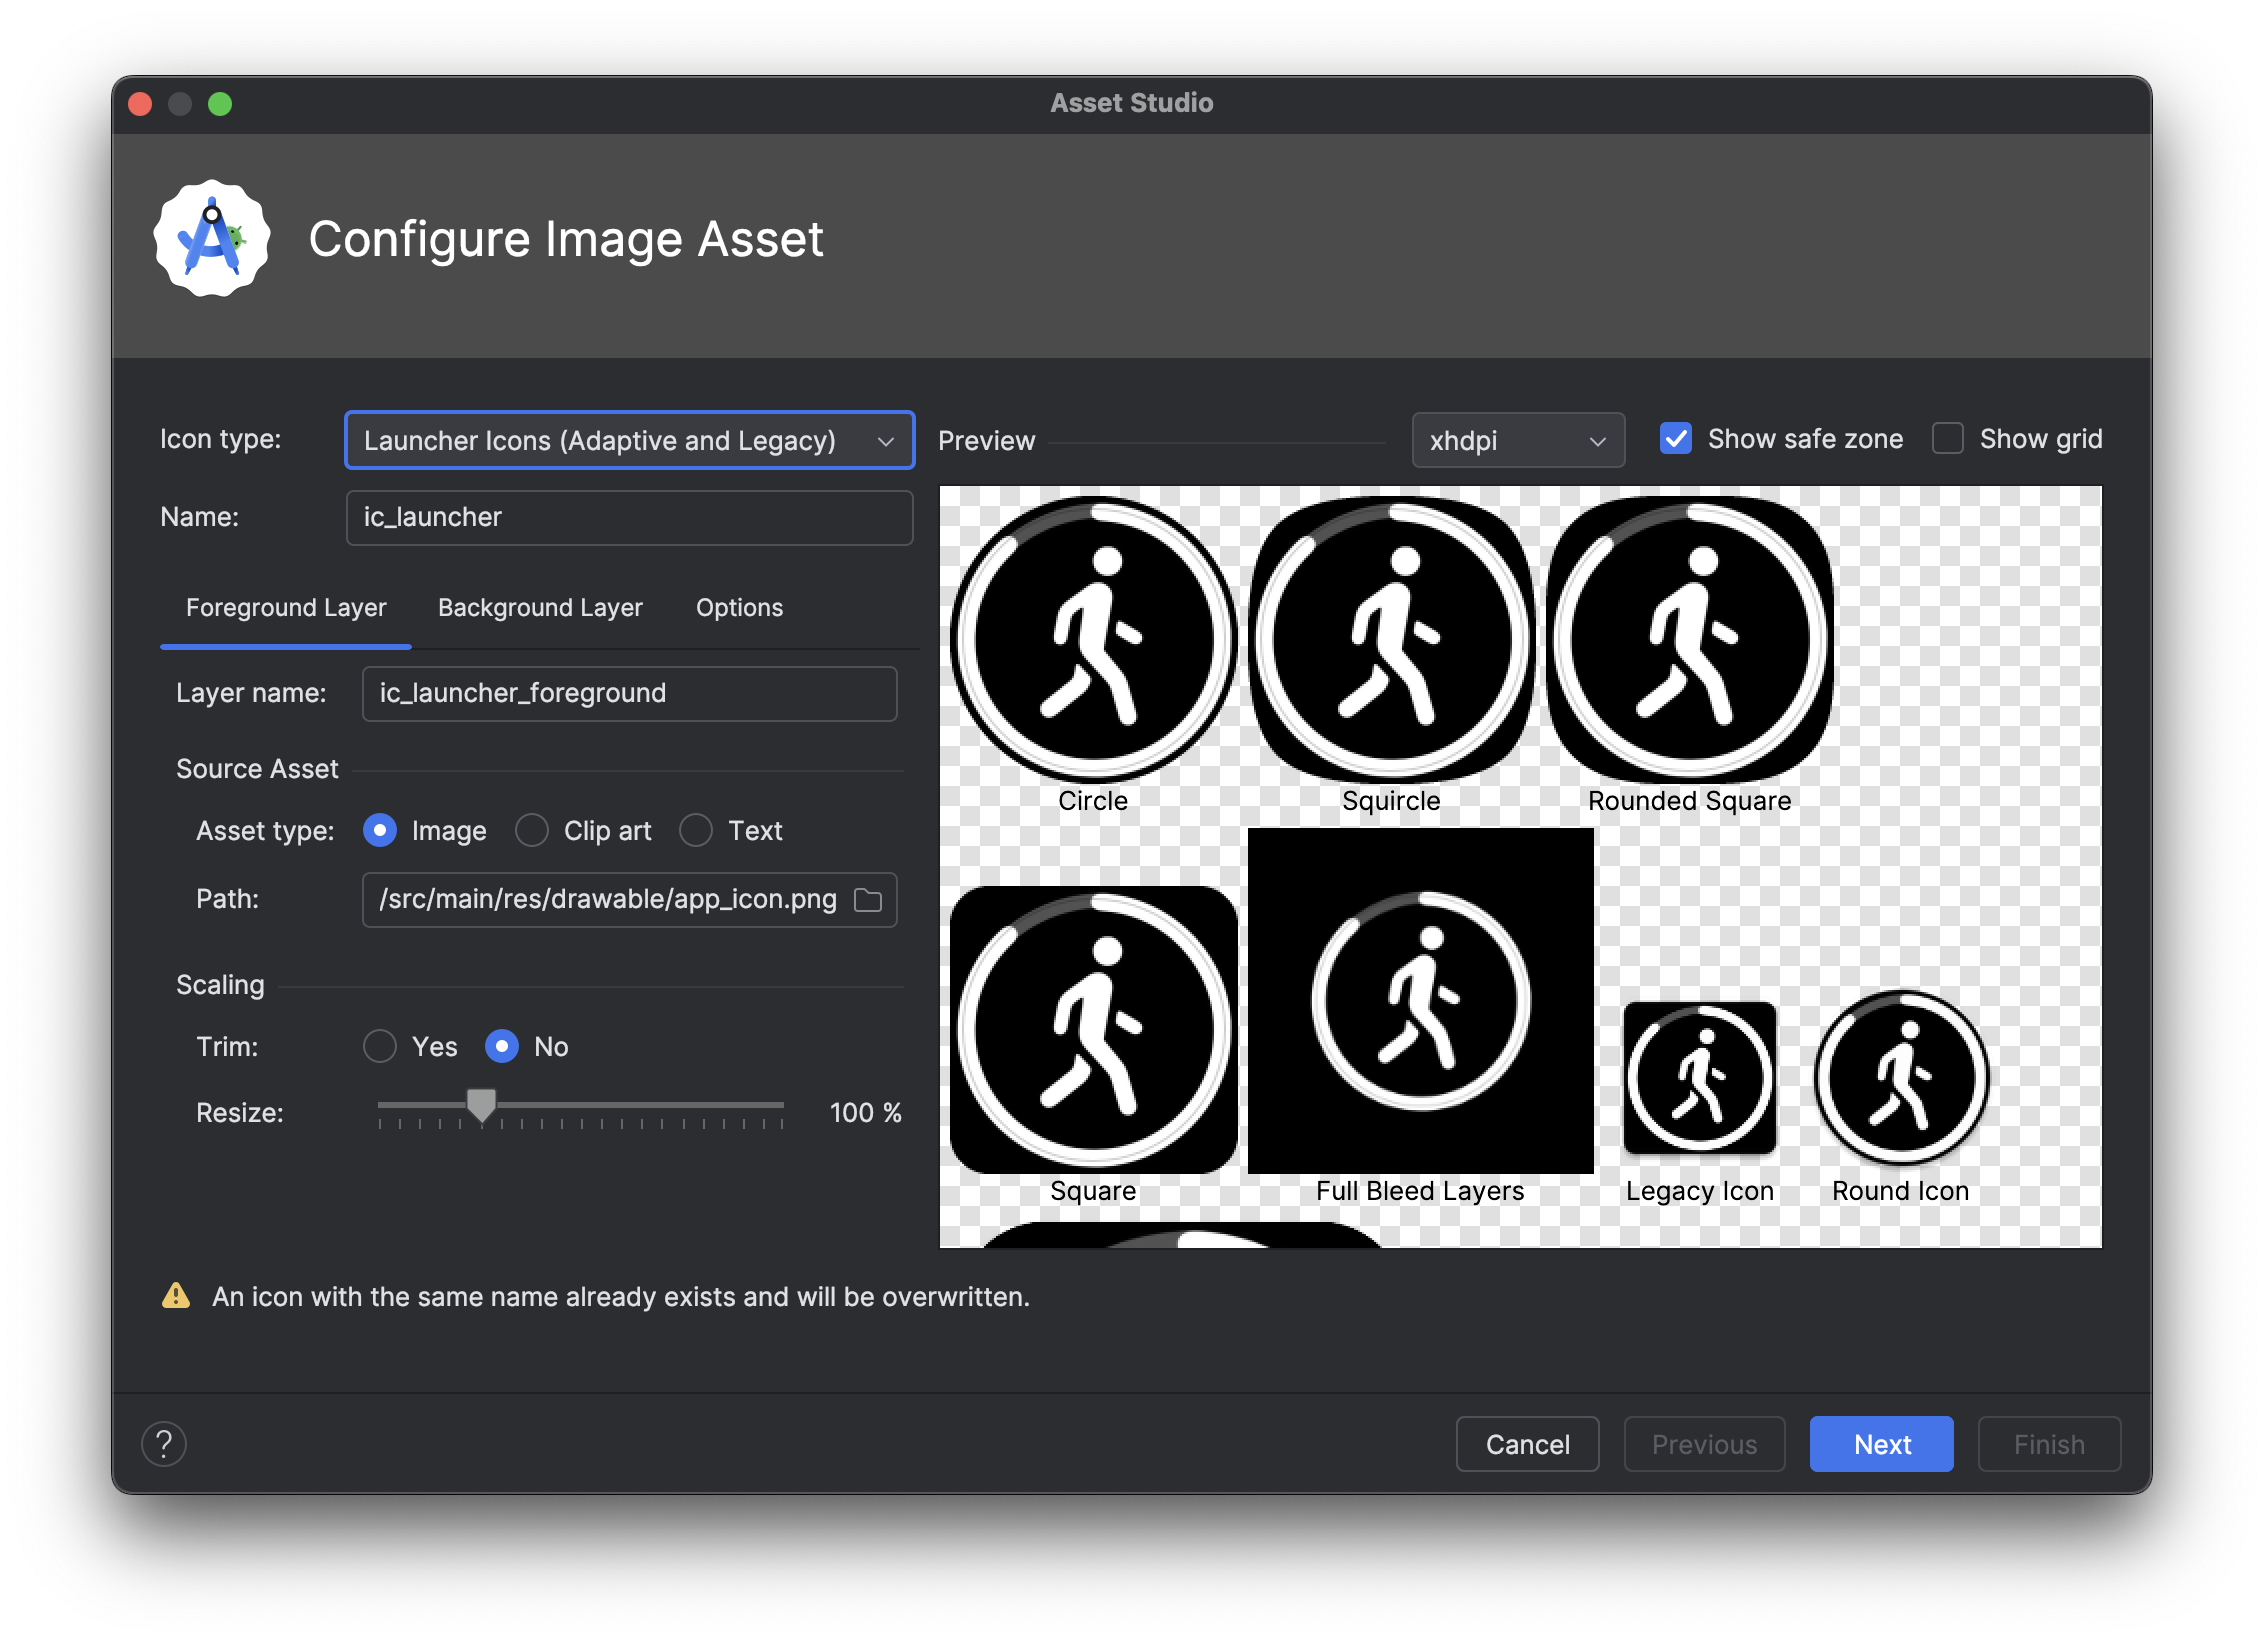
\includegraphics[width=0.5\textwidth]{res/img/appIcon.png}
            \caption{Generating Icons in Android Studio}
            \label{fig:ex2_1.1}
        \end{figure}
        
        Android Studio handled the generation of all necessary formats for the image, including various resolution sizes and shapes (see Figure~\ref{fig:ex2_2.2}).
        
        \begin{figure}[H]
            \centering
            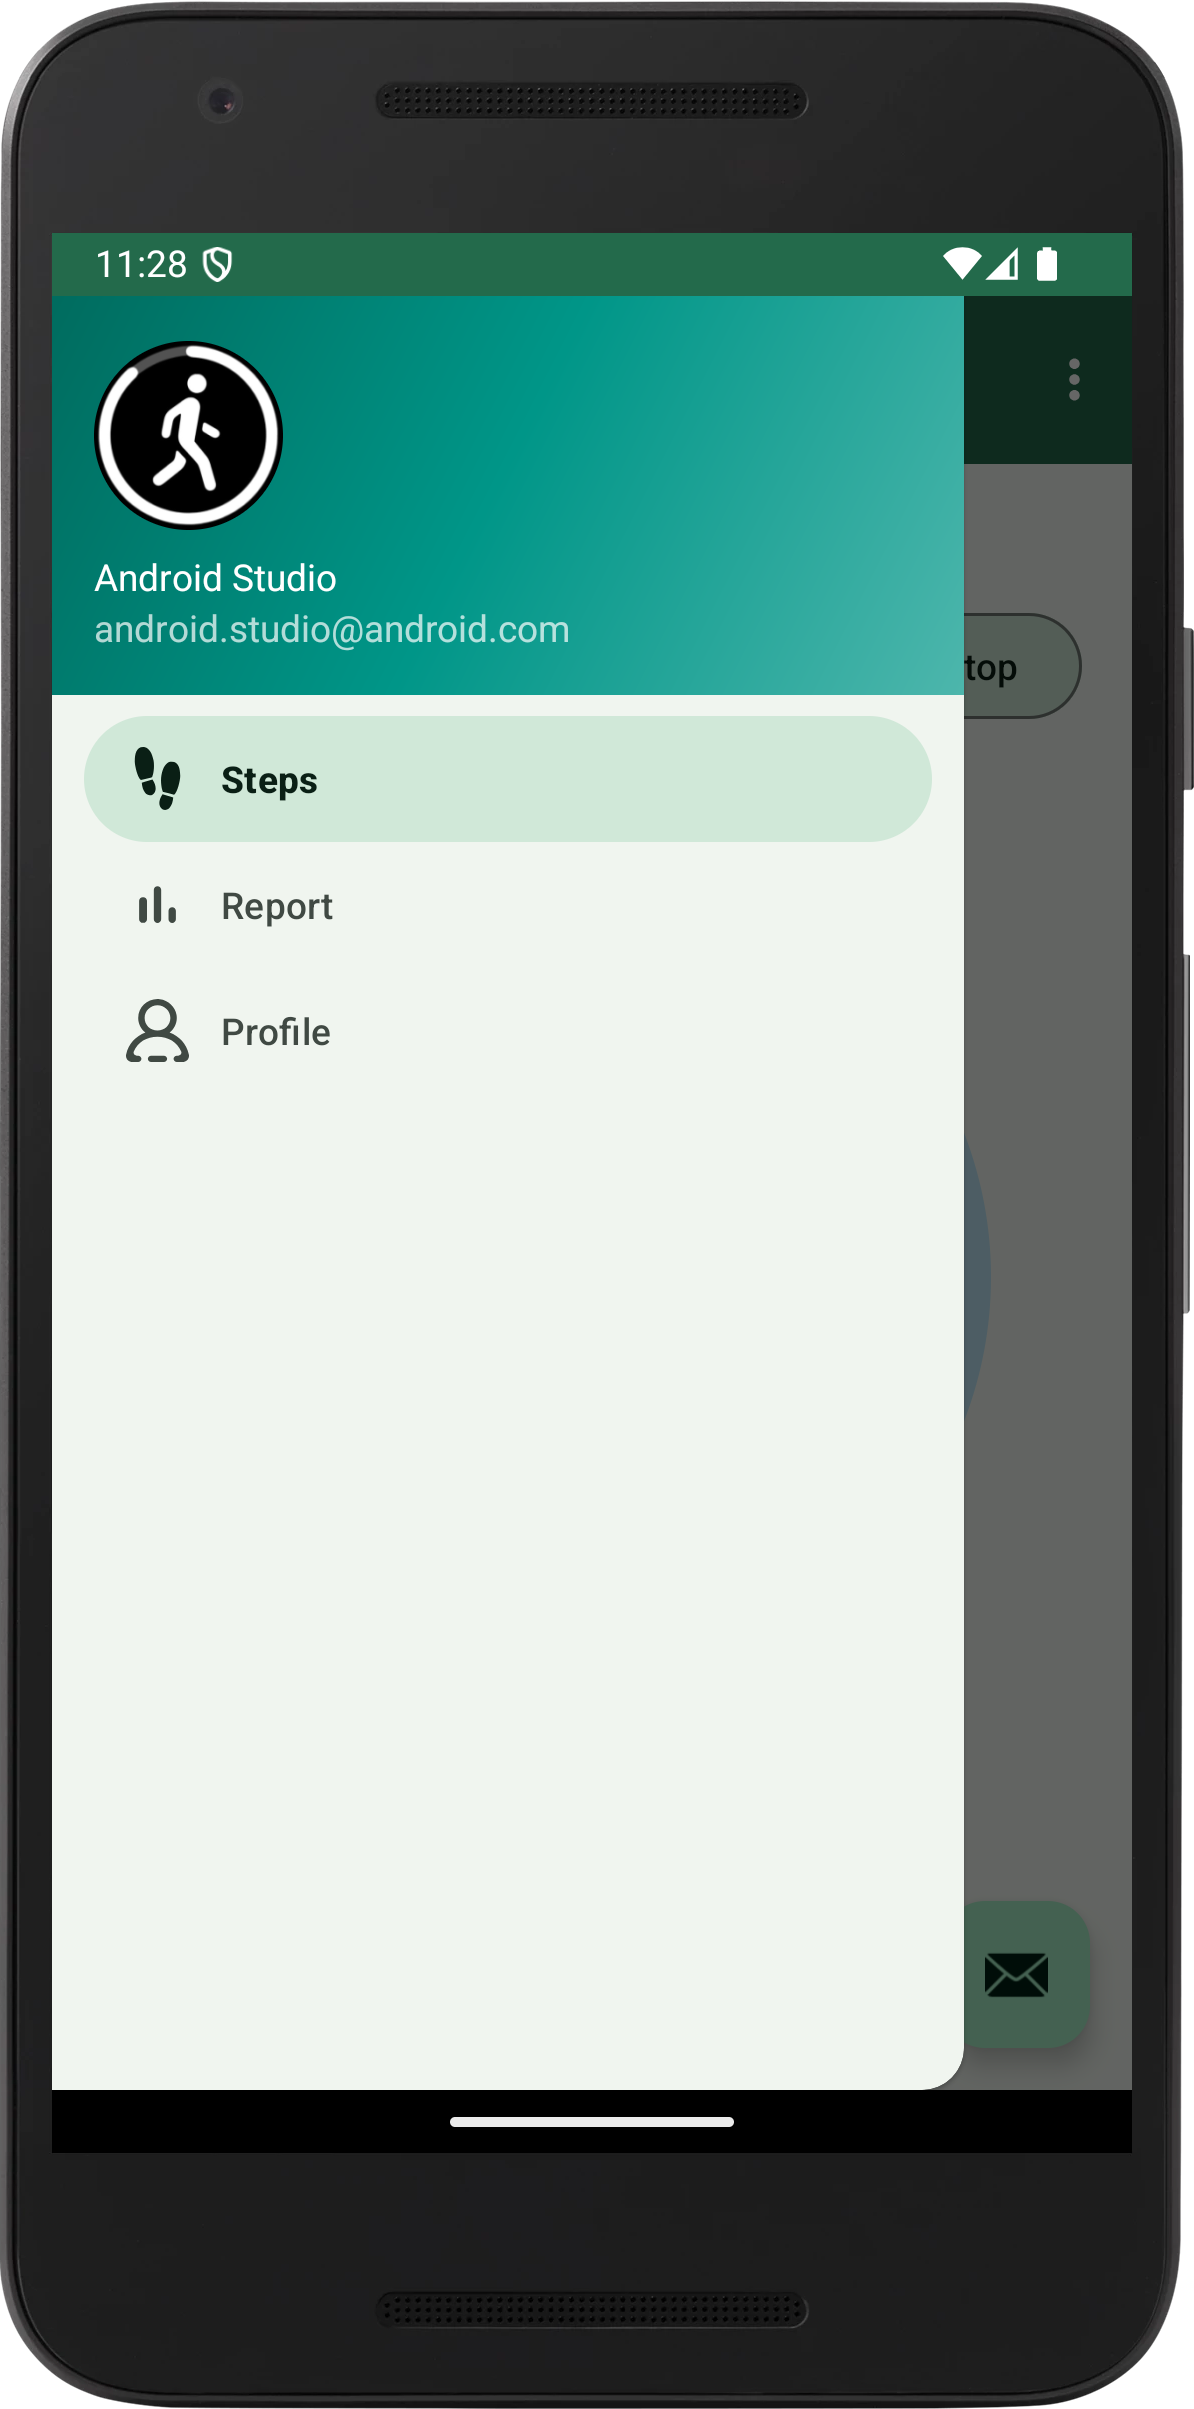
\includegraphics[width=0.20\textwidth]{res/img/icon1.png}
            \hspace{0.05\textwidth}
            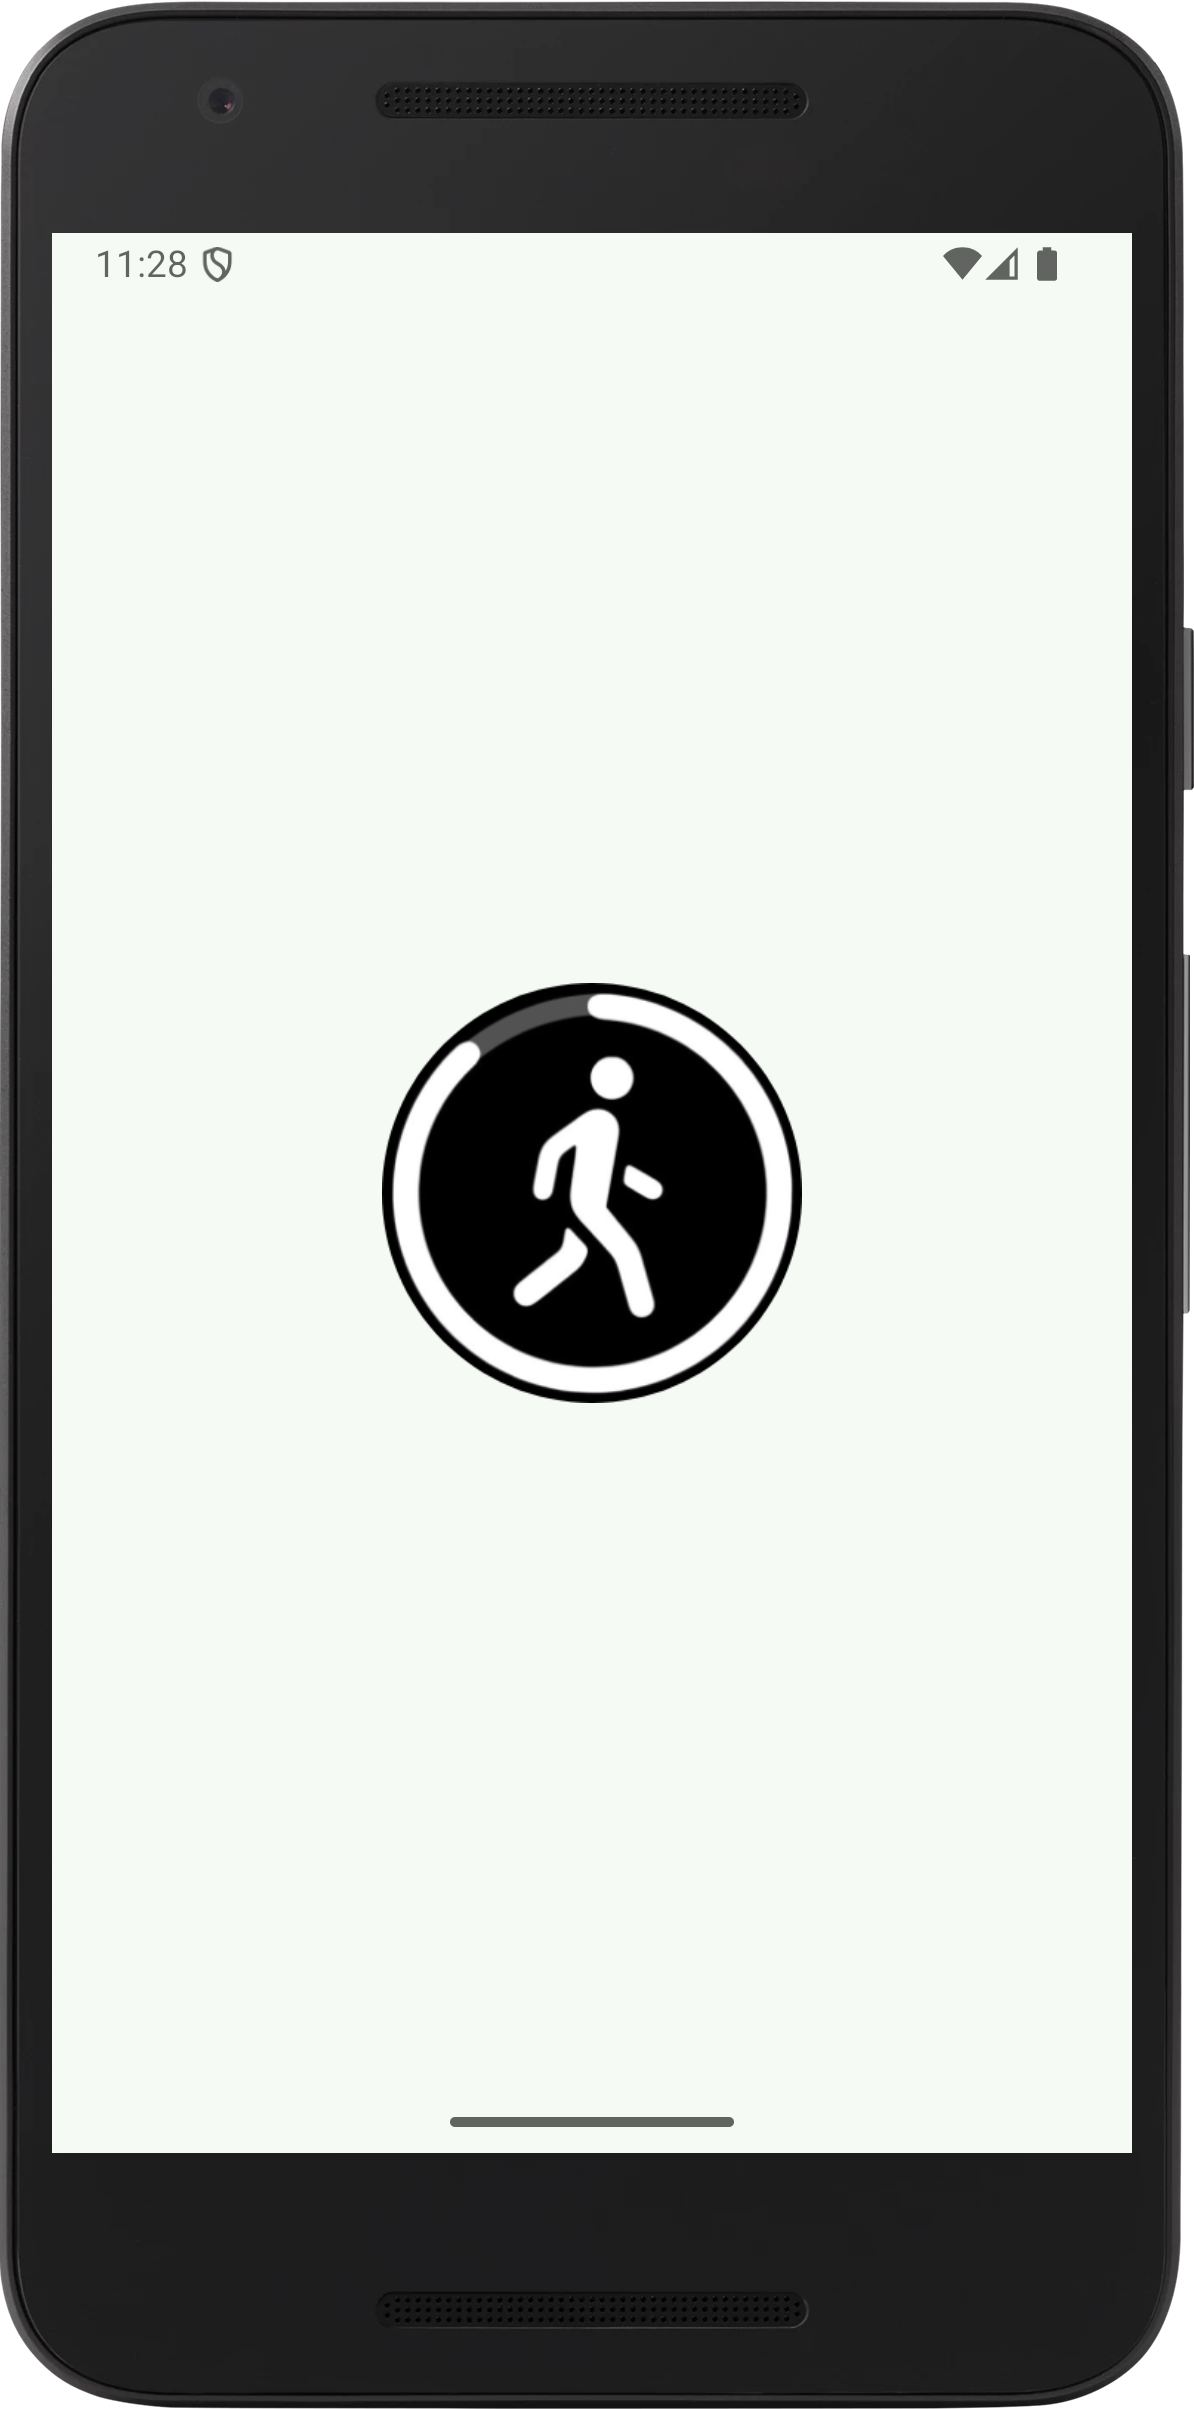
\includegraphics[width=0.20\textwidth]{res/img/icon2.png}      
            \hspace{0.05\textwidth}
            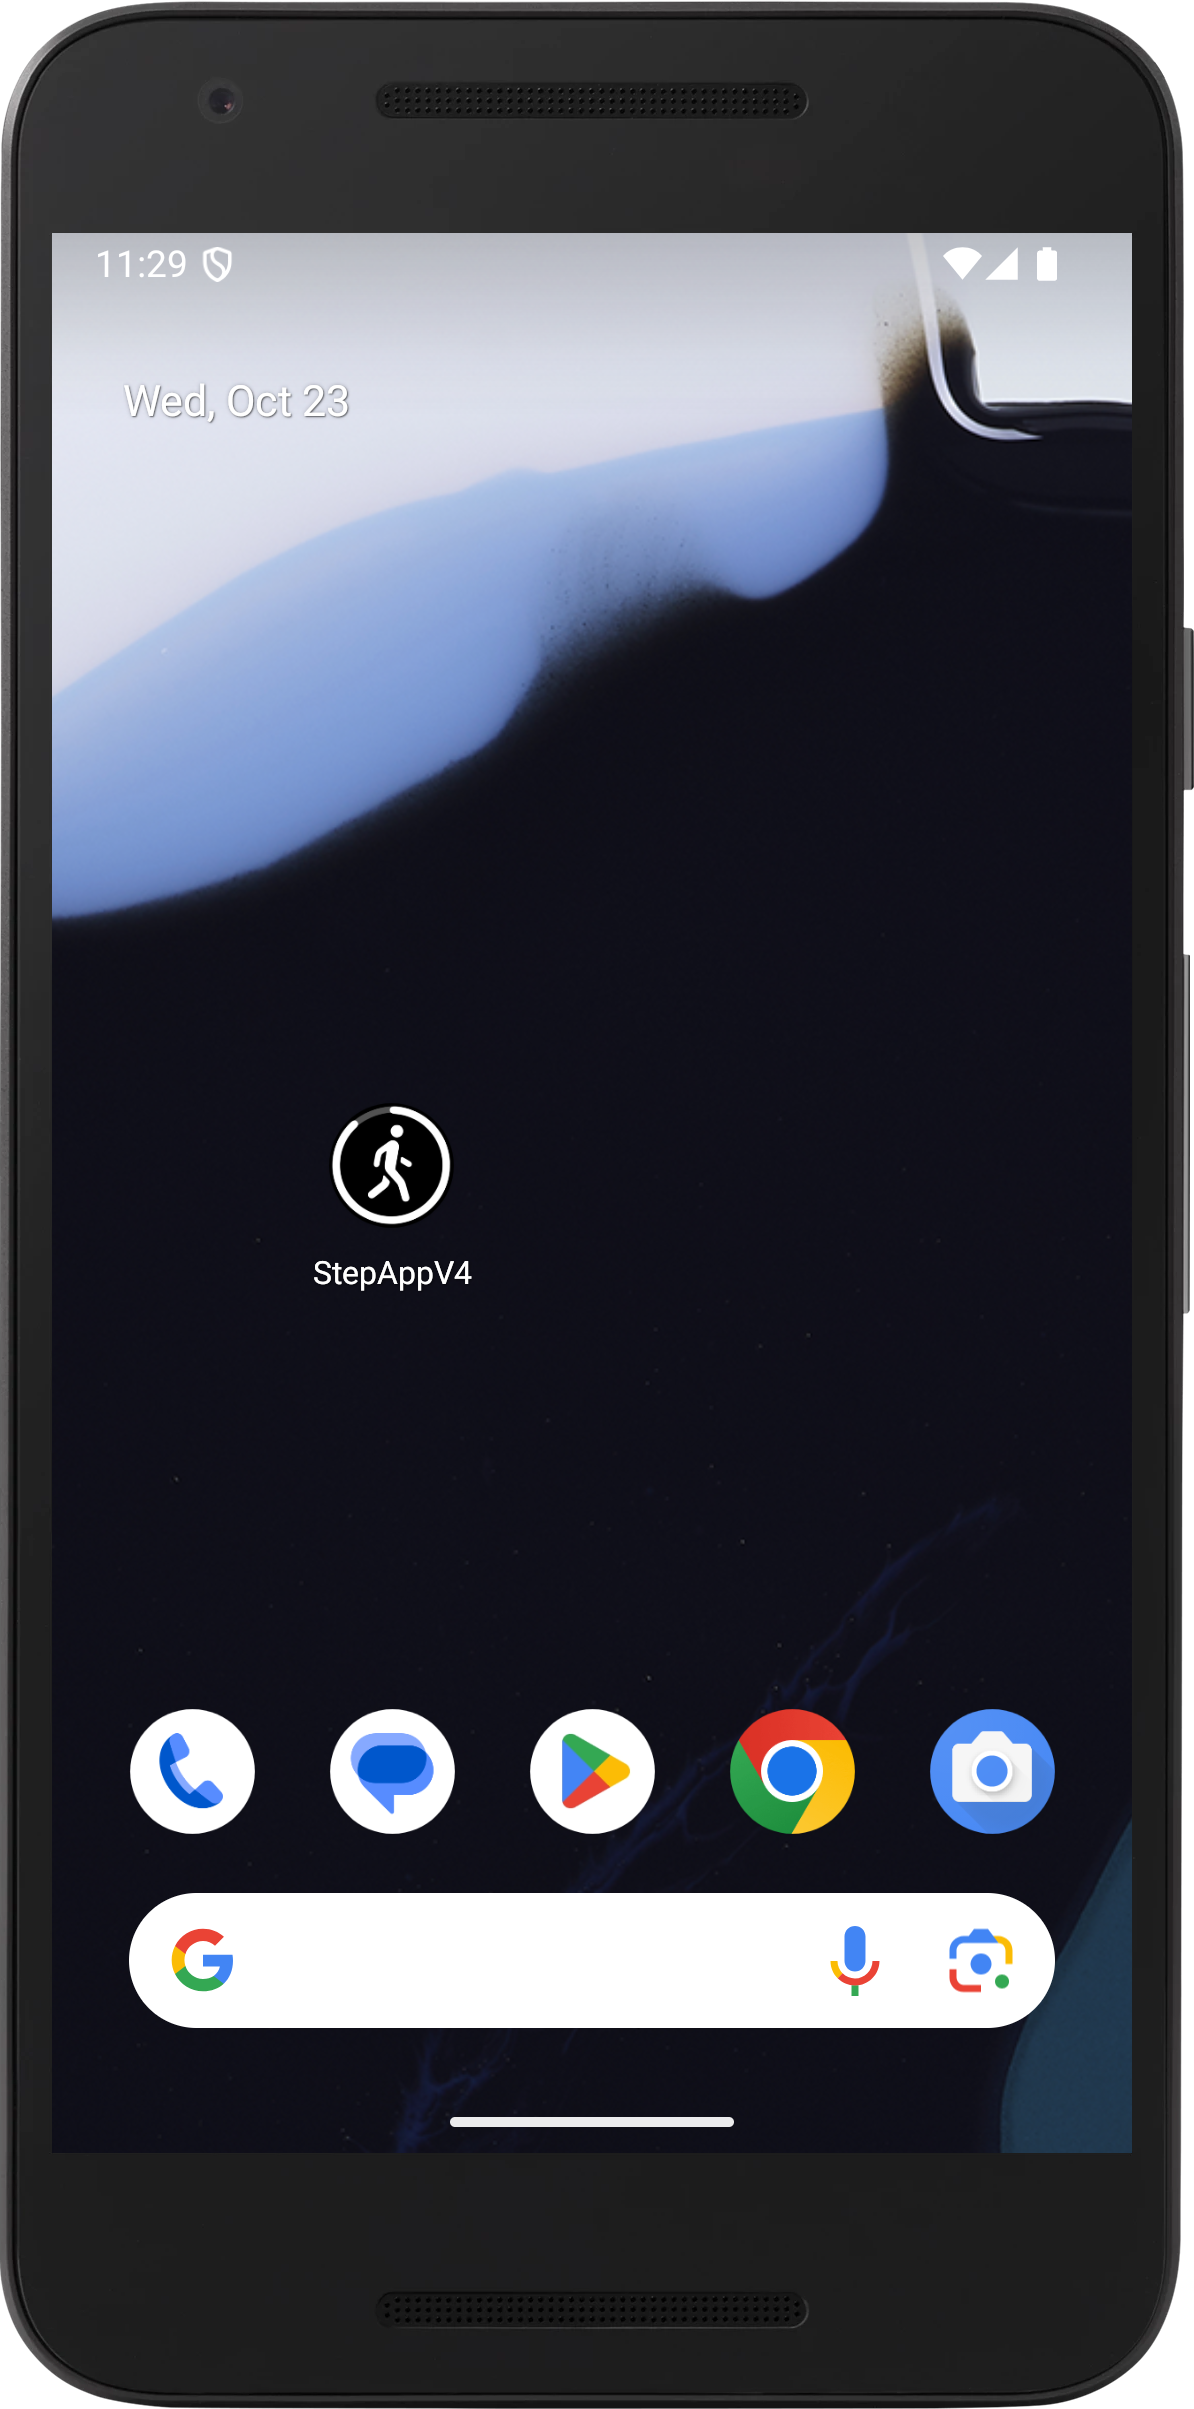
\includegraphics[width=0.20\textwidth]{res/img/icon3.png}
            \caption{Generated Icons with Different Resolutions and Shapes}
            \label{fig:ex2_2.2}
        \end{figure}



\newpage


\subsection{Implement Dark Theme}
    To implement the dark theme, I utilized the \texttt{AppCompatDelegate} class provided by Android's support library. This allows for easy switching between light and dark modes. The dark mode can be toggled by the user via a switch placed in the \texttt{Profile} page (see Figure~\ref{fig:ex2_3}).

    \begin{figure}[H]
        \centering
        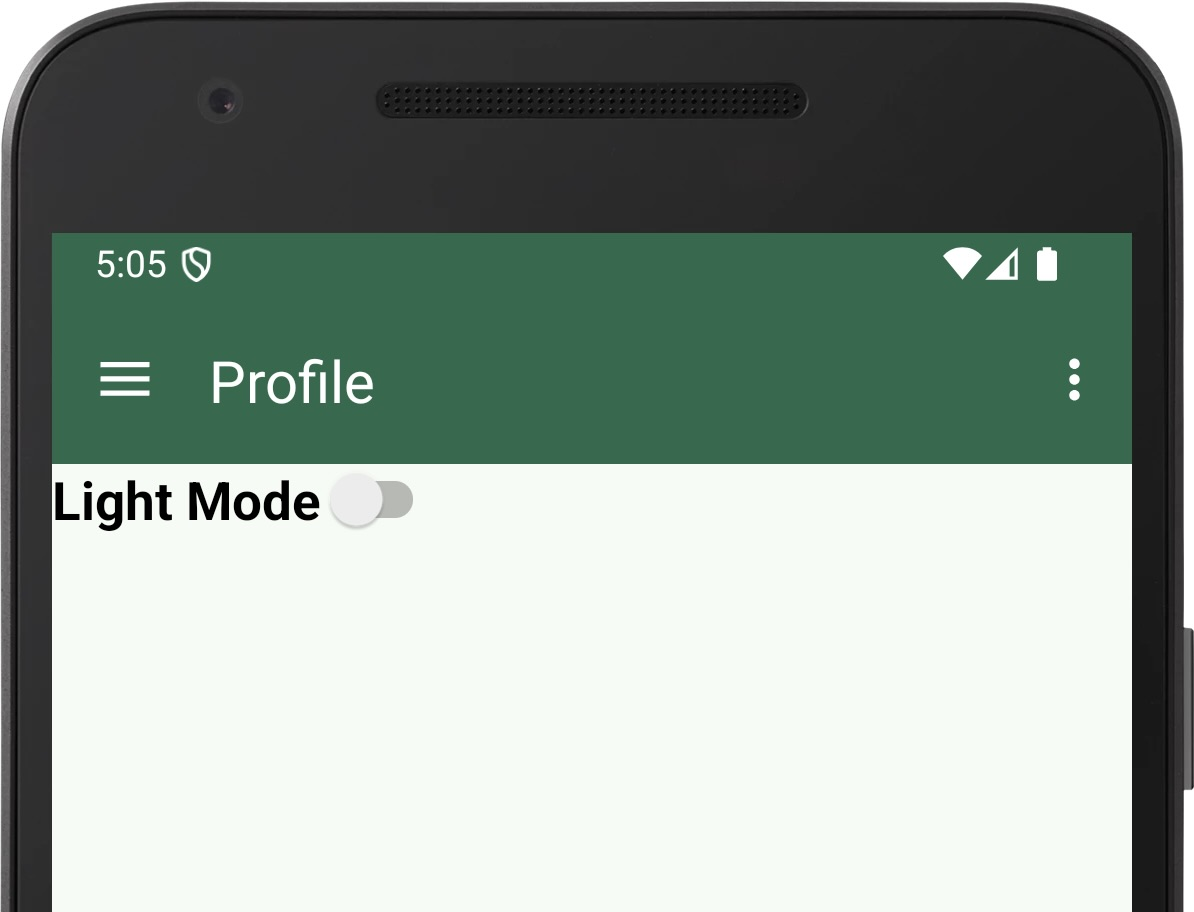
\includegraphics[width=0.2\textwidth]{res/img/dark_theme_switch.png}
        \caption{Switch for toggling between Light and Dark Modes}
        \label{fig:ex2_3}
    \end{figure}

    The dark mode implementation involved modifying the \texttt{ProfileFragment} and adding an \\ \texttt{OnCheckedChangeListener} to the switch. Depending on whether the switch is checked or not, the theme is switched using \texttt{AppCompatDelegate.setDefaultNightMode()}. If the switch is turned on, the dark theme is enabled using \texttt{AppCompatDelegate.MODE\_NIGHT\_YES}, and if the switch is off, the light theme is restored using \texttt{AppCompatDelegate.MODE\_NIGHT\_NO}.

    The relevant code for the theme switching logic is shown below:

    \lstinputlisting[firstline=45]{../app/src/main/java/com/example/stepappv4/ui/slideshow/ProfileFragment.java}

    Additionally, I ensured that the \texttt{colors.xml} file contained separate color definitions for both light and dark modes . This file is located in the \texttt{res/values} and \texttt{res/values-night} directories for light and dark modes, respectively. Same thing I had to do for the Themes, this prevented the app from changing layout changes. The following figures are some screenshots of the app in dark mode (see Figure~\ref{fig:ex2_2.4}).

    \begin{figure}[H]
        \centering
        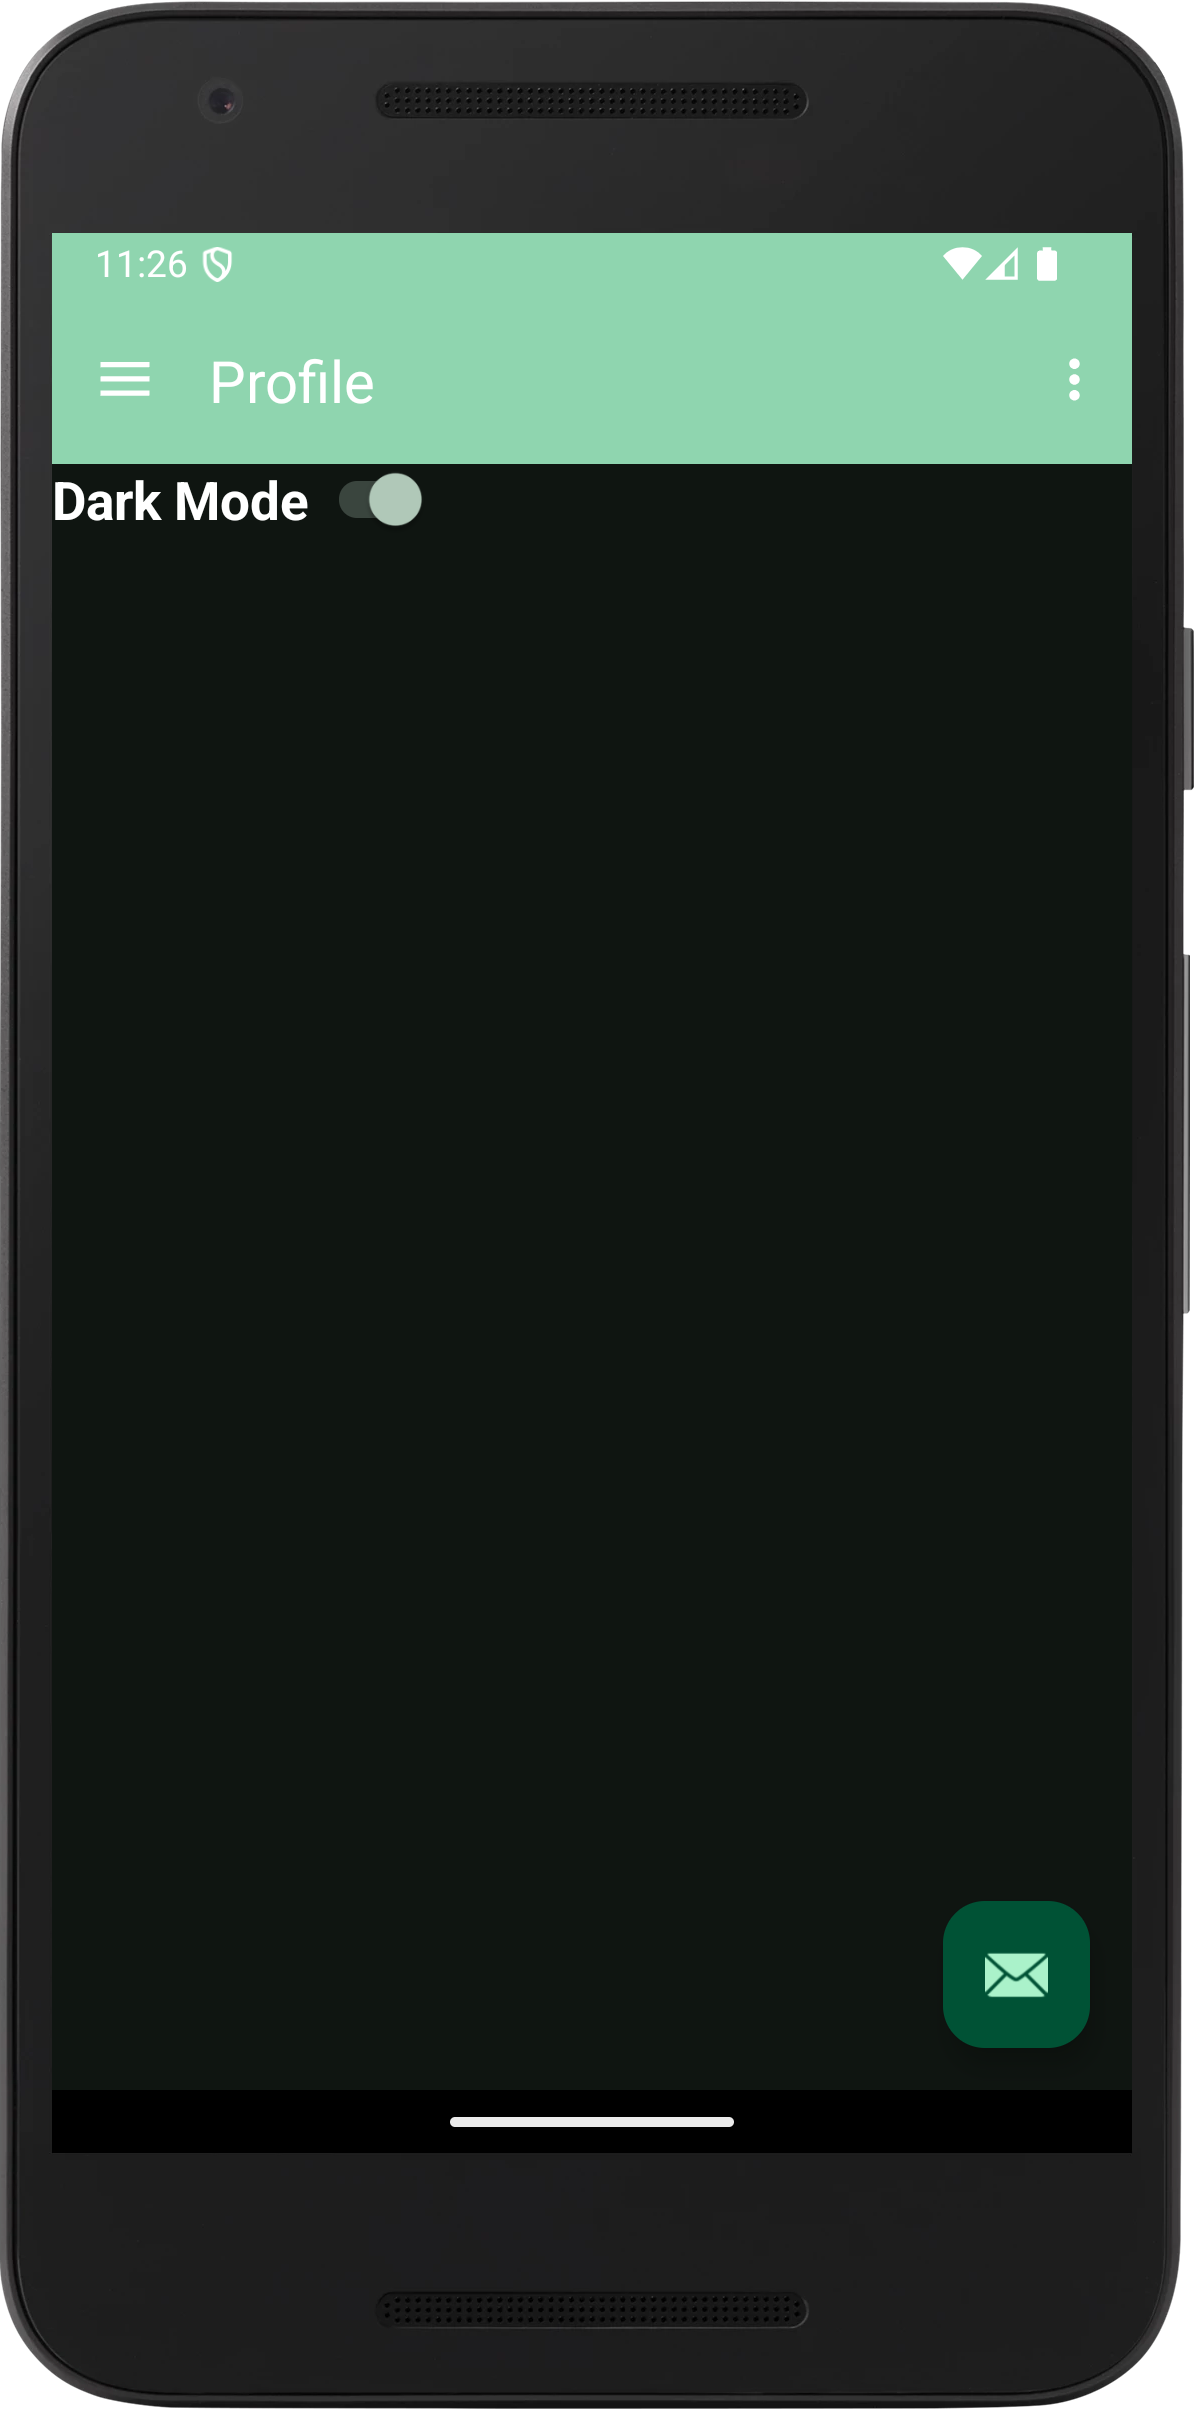
\includegraphics[width=0.20\textwidth]{res/img/darkMode1.png}
        \hspace{0.05\textwidth}
        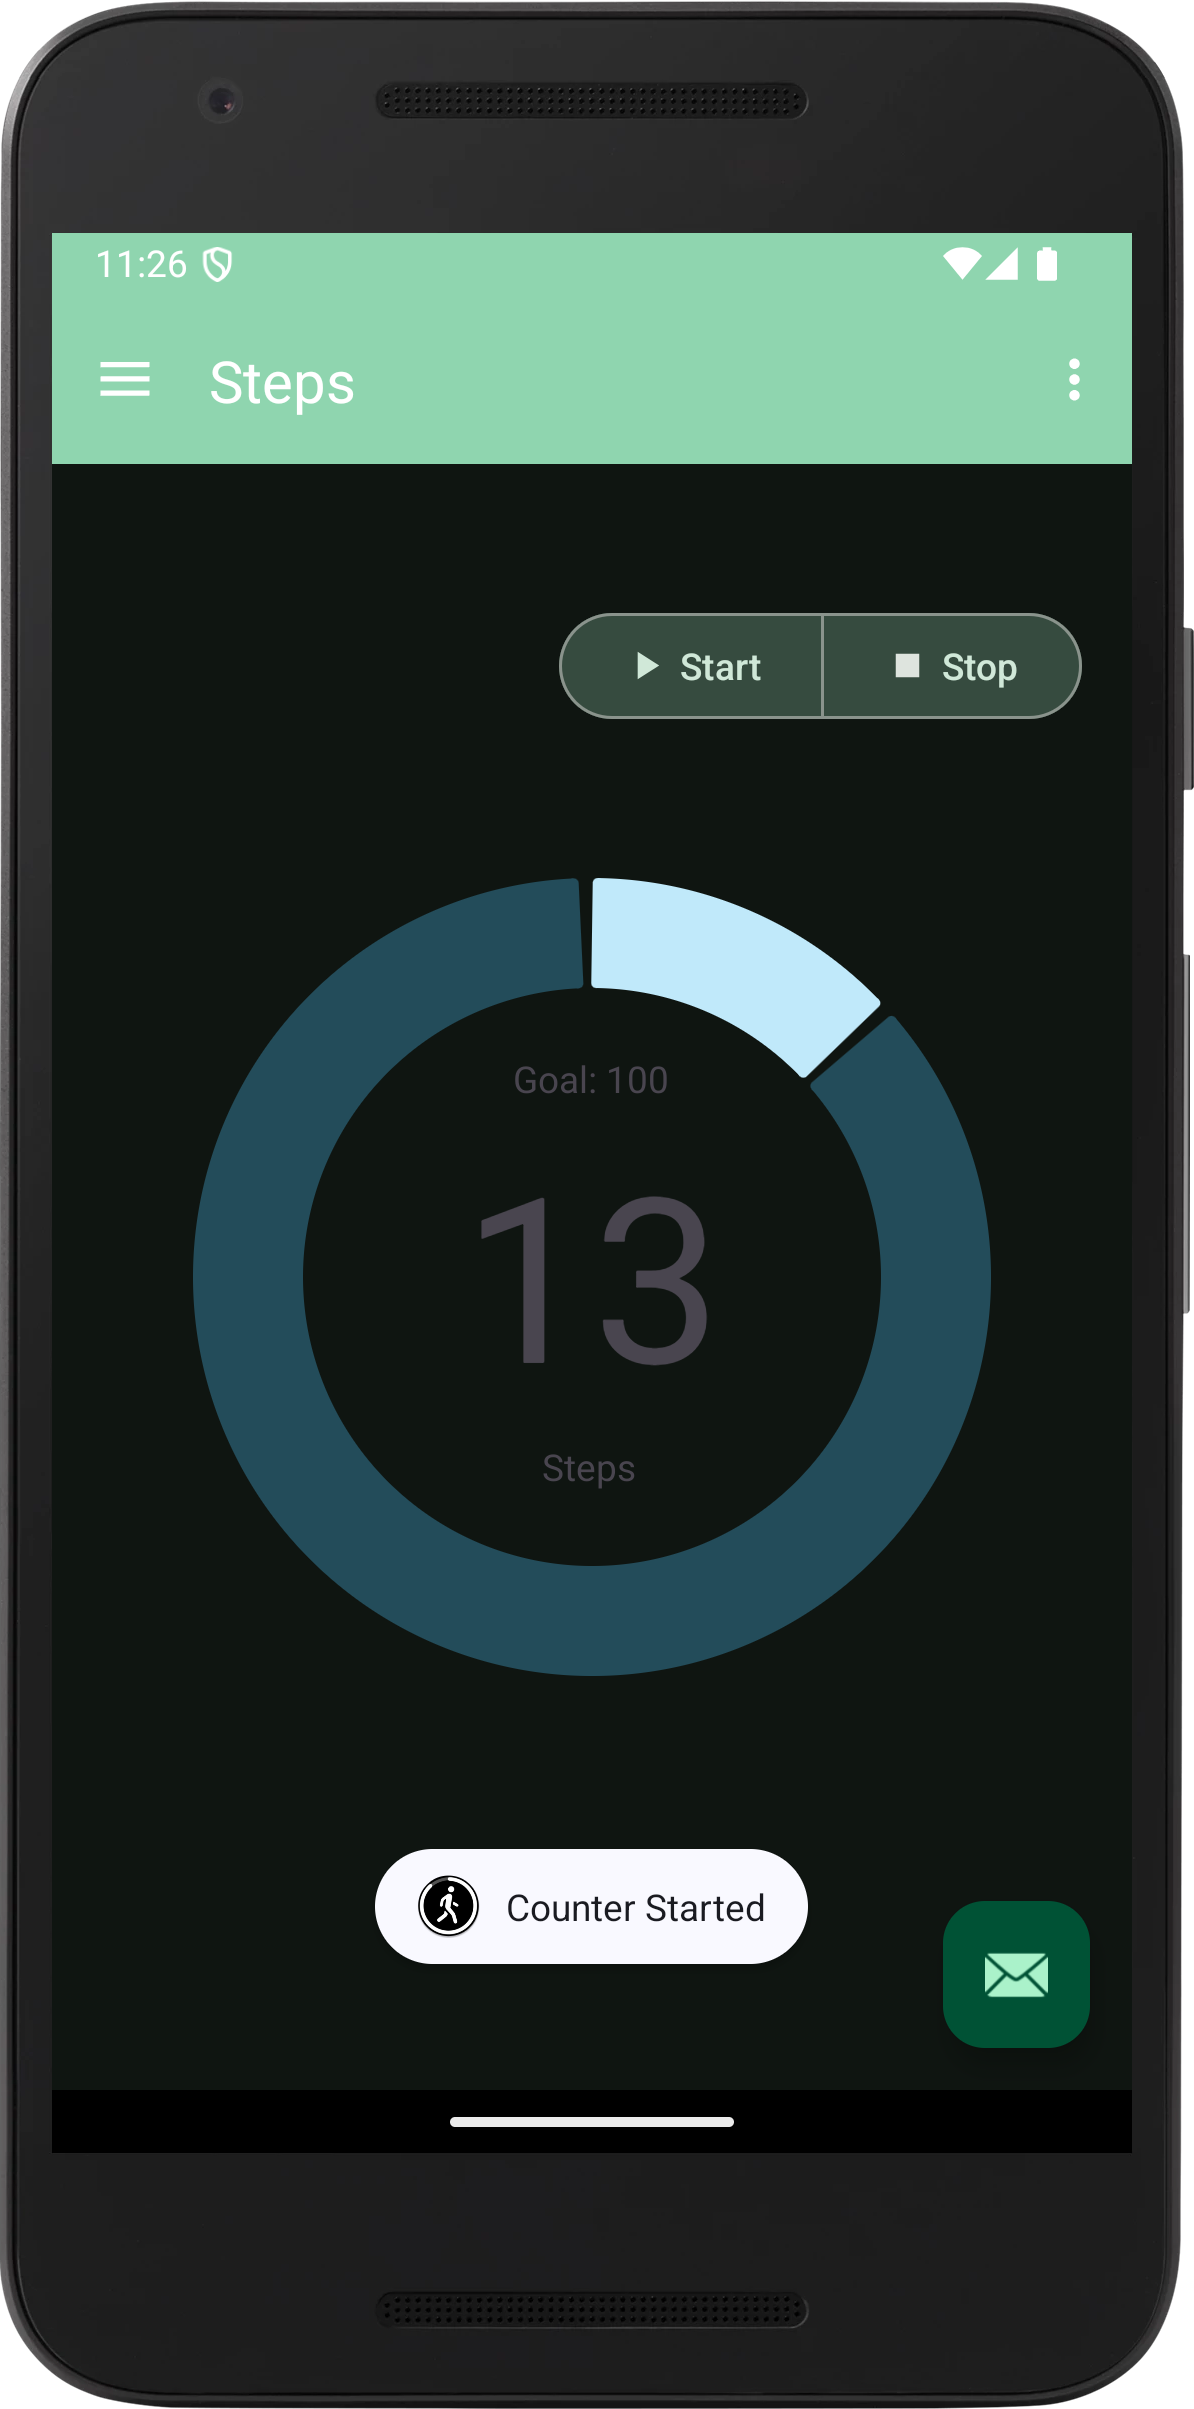
\includegraphics[width=0.20\textwidth]{res/img/darkMode2.png}      
        \hspace{0.05\textwidth}
        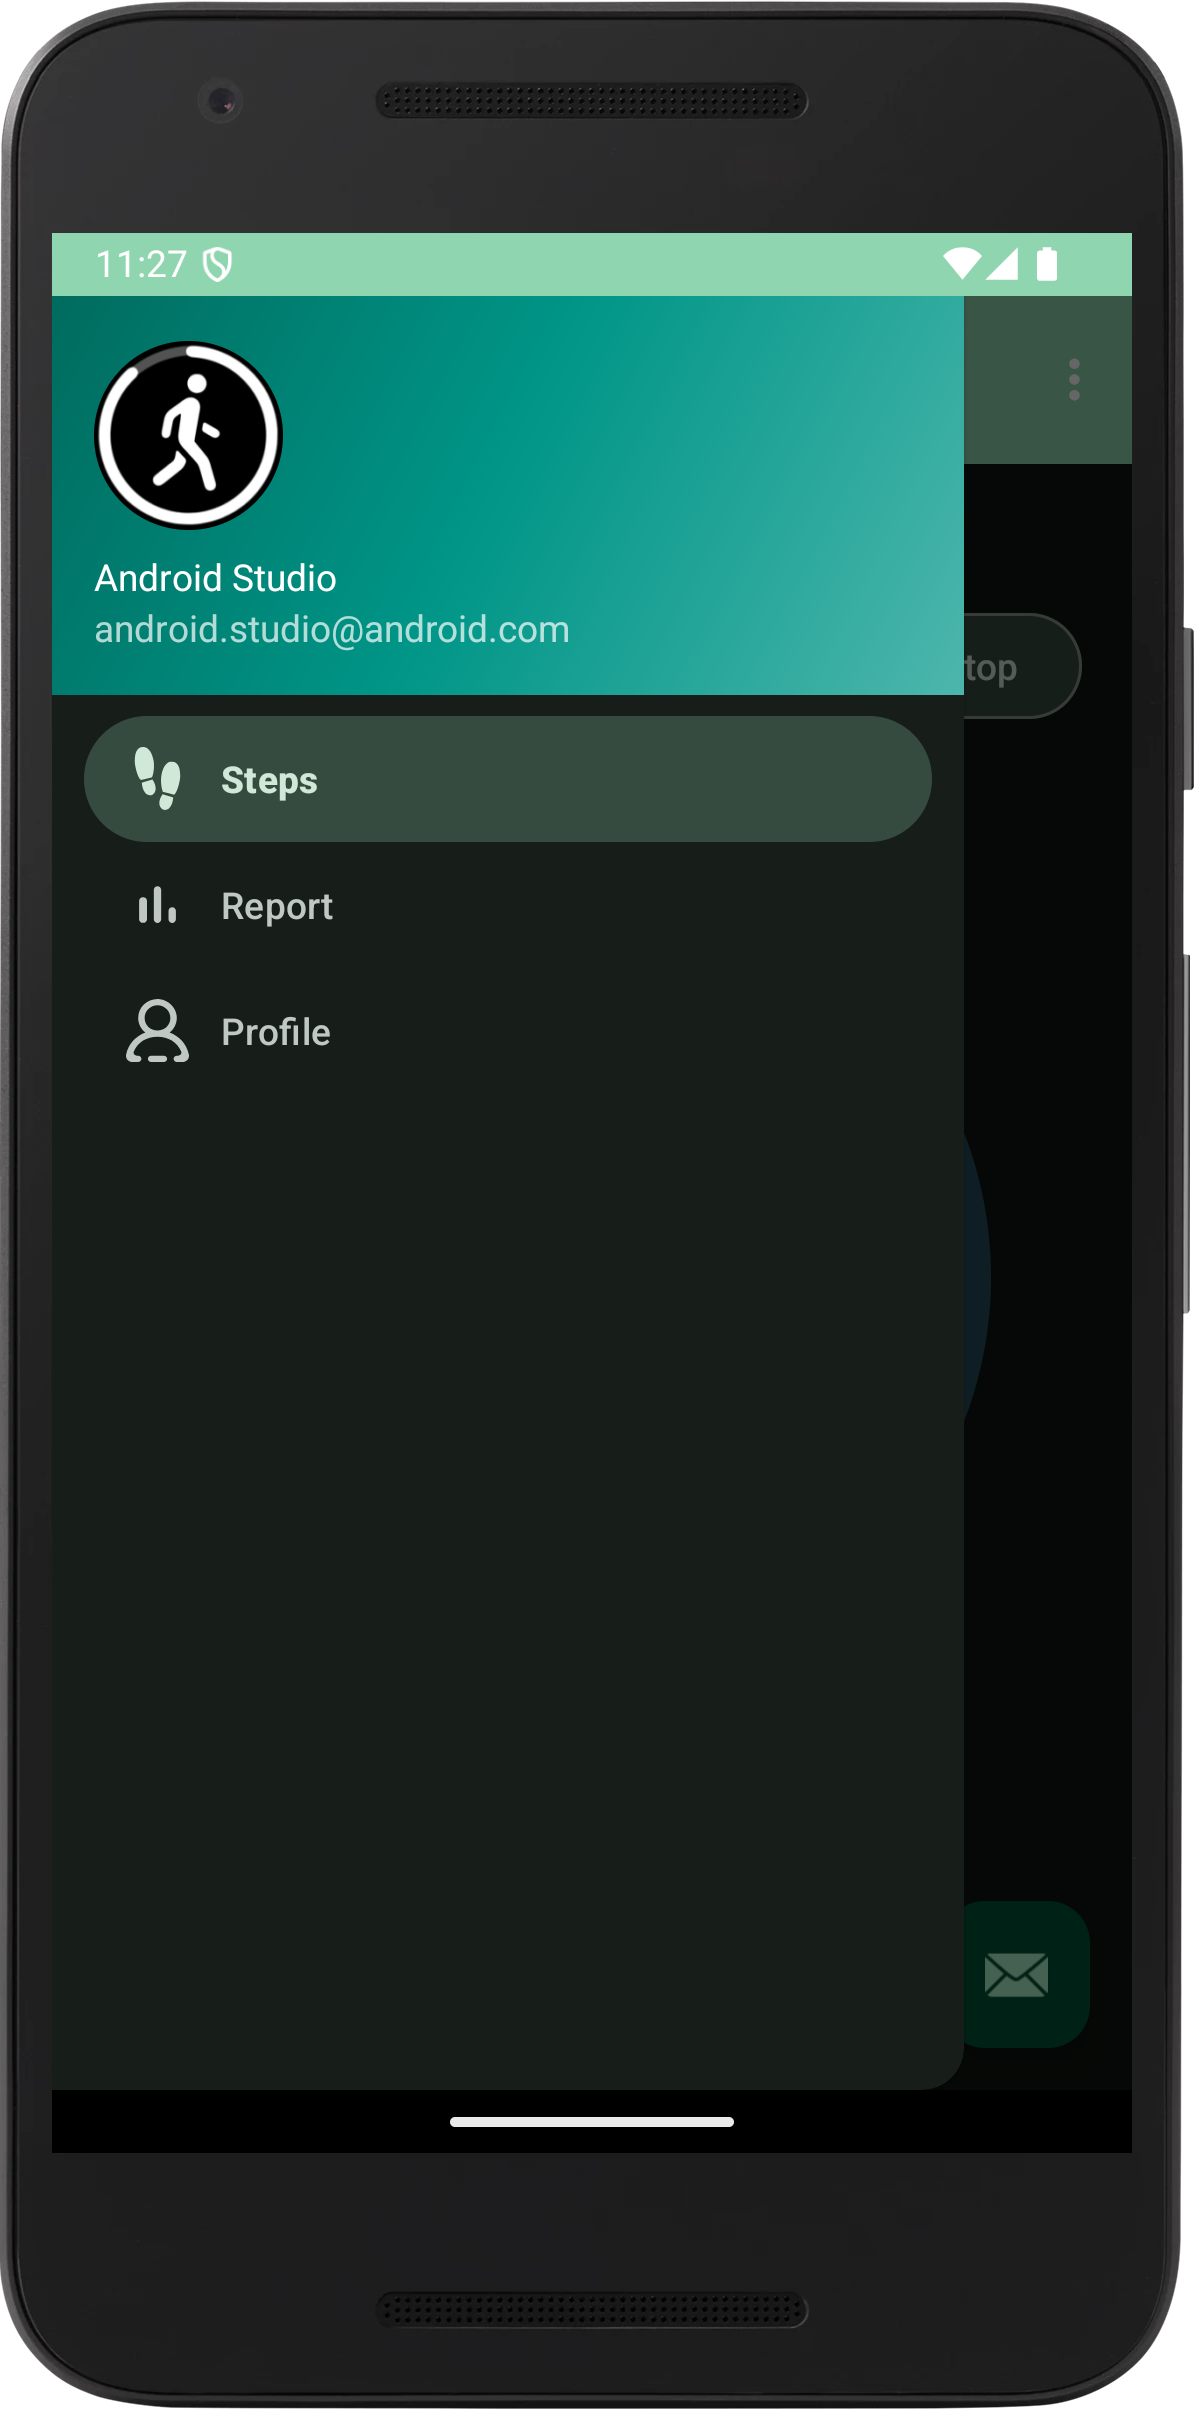
\includegraphics[width=0.20\textwidth]{res/img/darkMode3.png}
        \caption{Generated Icons with Different Resolutions and Shapes}
        \label{fig:ex2_2.4}
    \end{figure}